
%(BEGIN_QUESTION)
% Copyright 2010, Tony R. Kuphaldt, released under the Creative Commons Attribution License (v 1.0)
% This means you may do almost anything with this work of mine, so long as you give me proper credit

Suppose we have a Siemens S7-200 PLC connected to a pair of process switches and light bulbs as shown in this illustration:

$$\includegraphics[width=15.5cm]{i04631x01.eps}$$

Examine the following relay ladder logic (RLL) program for this Siemens PLC, determining the statuses of the two lamps provided the pressure switch sees a fluid pressure of 30 PSI and the level switch sees a liquid level of 4 feet:

$$\includegraphics[width=15.5cm]{i04631x02.eps}$$

\underbar{file i04631}
%(END_QUESTION)





%(BEGIN_ANSWER)

Green lamp is on, red lamp is off.

%(END_ANSWER)





%(BEGIN_NOTES)


%INDEX% PLC, relating I/O status to virtual elements

%(END_NOTES)


